\chapter{Basic Concepts}

\section{Analytic Functions}

\begin{definition}[{[Connected and Simply Connected Regions] [1]}]
	In the complex plane \(\C\), a subset \(\varepsilon \subset \C\) is called a \emph{connected region} (or simply a \emph{domain}) if it is open and any two points in \(\varepsilon\) can be joined by a polygonal path (in particular, a straight-line path) lying entirely within \(\varepsilon\).
	
	A region \(\varepsilon\) is said to be \emph{simply connected} if it is connected and its complement \(\varepsilon^{c} = \C \setminus \varepsilon\) is also connected. Equivalently, every closed curve in \(\varepsilon\) can be continuously deformed to a point while remaining inside \(\varepsilon\).
\end{definition}

\begin{figure}[ht]
	\centering
	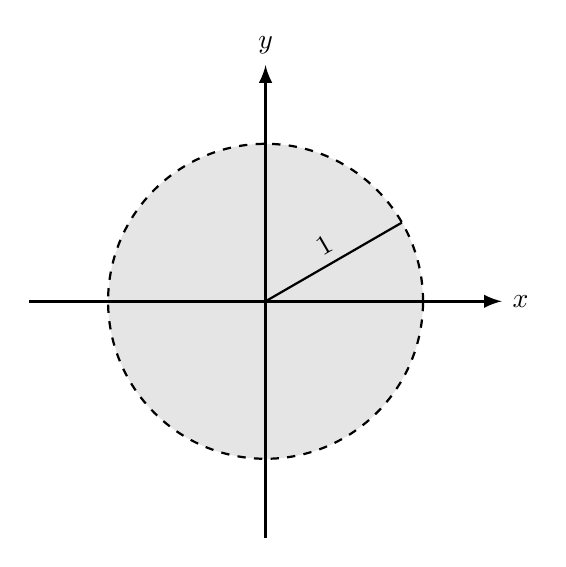
\begin{tikzpicture}[scale=2]
		\fill[gray!20] (0,0) circle (1);
		
		% Axes
		\draw[-latex, very thick] (-1.5,0) -- (1.5,0) node[right] {$x$};
		\draw[-latex, very thick] (0,-1.5) -- (0,1.5) node[above] {$y$};
		
		% Filled unit disk
		\draw[thick] (0, 0) -- ++(30:1) node[above, midway, sloped]{$1$};
		
		% Boundary circle
		\draw[thick, black, dashed] (0,0) circle (1);
		
		% Label
		\node at (1,1) {$\U$};
	\end{tikzpicture}
	\caption{The region $\U = \{z : |z| < 1\}$}
\end{figure}



\begin{definition}[{[Analytic (Holomorphic) Function]}]
	A function \(f : \C \to \C\) is said to be \emph{analytic} (or \emph{holomorphic}) at a point \(z_0 \in \C\) if it is differentiable in some neighborhood of \(z_0\). That is, the limit
	\begin{equation}\label{eq:def-derivative}
		f'(z_0) = \lim_{\Delta z \to 0} \frac{f(z_0 + \Delta z) - f(z_0)}{\Delta z}
	\end{equation}
	exists.
	
	If \(f\) is analytic at every point of the open disc
	\[
	\U_r(z_0) = \{\, z \in \C : |z - z_0| < r \,\},
	\]
	then we say that \(f\) is analytic in \(\U_r(z_0)\). In such a disc, an analytic function admits a Taylor series expansion:
	\begin{equation}\label{eq:taylor}
		f(z) = \sum_{k=0}^{\infty} a_k (z - z_0)^k, 
		\qquad 
		a_k = \frac{f^{(k)}(z_0)}{k!},
	\end{equation}
	and this series converges to \(f(z)\) for every \(z \in \U_r(z_0)\).
\end{definition}

\begin{figure}[ht]
	\centering
	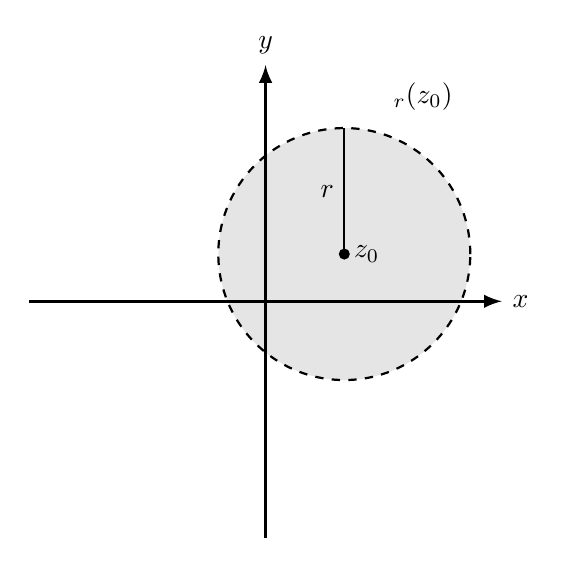
\begin{tikzpicture}[scale=2]
		% Define center and radius
		\def\xo{0.5}
		\def\yo{0.3}
		\def\r{0.8}
		
		% Filled disk
		\fill[gray!20] (\xo,\yo) circle (\r);
		
		% Axes
		\draw[-latex, very thick] (-1.5,0) -- (1.5,0) node[right] {$x$};
		\draw[-latex, very thick] (0,-1.5) -- (0,1.5) node[above] {$y$};
		
		% Boundary circle
		\draw[thick, dashed] (\xo,\yo) circle (\r);
		
		% Center point
		\fill (\xo,\yo) circle (1pt);
		\node[right] at (\xo,\yo) {$z_0$};
		
		\draw[thick] (\xo,\yo) -- ++(90:\r) node[midway, left] {$r$};
		
		% Label
		\node at (1,1.3) {$\U_r(z_0)$};
	\end{tikzpicture}
	\caption{The region $\U_r = \{z : | z - z_0 | < r\}$}
\end{figure}

\section{Some Classes of Analytic Functions}

\subsection[The Class \(\mathcal{A}\)]{The Class \(\mathcal{A}\) [1]}

Let \(\U = \{ z \in \C : |z| < 1 \}\) denote the open unit disc.  
The class \(\mathcal{A} = \mathcal{A}(\U)\) consists of all functions \(f\) analytic in \(\U\) that satisfy the normalization conditions
\[
f(0) = 0, 
\qquad 
f'(0) = 1.
\]
Consequently, every \(f \in \mathcal{A}\) admits the Taylor expansion
\[
f(z) = z + \sum_{k=2}^{\infty} a_k z^k.
\]

\newpage

\subsection[The Class \(\varphi\)]{The Class \(\varphi\) [3]}

Let \(\varphi\) denote the class of analytic functions in the unit disc whose real part is positive:
\[
\varphi = \{\, \omega : \U \to \C 
\;\text{analytic},\; 
\re(\omega(z)) > 0 \text{ for all } z \in \U \,\}.
\]
A function \(\omega \in \varphi\) is typically normalized by
\[
\omega(0) = 1,
\]
and thus has the Taylor expansion
\[
\omega(z) = 1 + \sum_{k=1}^{\infty} w_k z^k.
\]

A classical example of a function in \(\varphi\) is
\[
\omega(z) = \frac{1 + z}{1 - z}
= 1 + 2z + 2z^2 + 2z^3 + \cdots
= 1 + \sum_{k=1}^{\infty} 2 z^k,
\]
which satisfies \(\re(\omega(z)) > 0\) for all \(z \in \U\).

Every function \(\omega \in \varphi\) can be expressed in terms of a function \(\Phi\) that is analytic in \(\U\), satisfies \(\Phi(0) = 0\), and maps \(\U\) into itself (that is, \( |\Phi(z)| < 1 \)).  
Such a function \(\Phi\), guaranteed by the Schwarz lemma, is referred to as a \emph{Schwarz function}.  
The representation takes the form
\begin{equation}\label{eq:cayley-transform}
	\omega(z) = \frac{1 + \Phi(z)}{1 - \Phi(z)}.
\end{equation}
This classical Cayley transform provides a complete characterization of all analytic functions with positive real part in the unit disc.
\newpage

\section[Univalent Functions]{Univalent Functions [1]}

The theory of univalent (i.e., one-to-one) analytic functions is a central part of geometric function theory.  
An analytic function
\[
f : \U \to \C, 
\qquad 
\U = \{ z \in \C : |z| < 1 \},
\]
is called \emph{univalent} if it is injective; that is,
\[
f(z_1) \neq f(z_2) \quad \text{whenever } z_1 \neq z_2.
\]

A particularly important subclass of univalent functions is the class \(S\), consisting of all functions analytic and univalent in \(\U\), normalized by
\[
f(0) = 0, 
\qquad 
f'(0) = 1.
\]
Thus every \(f \in S\) admits the Taylor expansion
\[
f(z) = z + a_2 z^2 + a_3 z^3 + \cdots.
\]

Several transformations preserve univalence and the normalization of the class \(S\).  
If \(f \in S\), then the following functions also belong to \(S\):

\begin{enumerate}
	\item \textbf{Rotation:}
	\[
	J(z) = e^{-i\theta} f(e^{i\theta} z),
	\qquad \theta \in \R.
	\]
	
	\item \textbf{Dilation:}
	\[
	J(z) = r^{-1} f(rz),
	\qquad 
	0 < r < 1.
	\]
	
	\item \textbf{Square-root transformation:}
	\[
	J(z) = \big(f(z^2)\big)^{1/2},
	\]
	which is analytic and univalent in \(\U\) with the appropriate branch of the square root.
	
	\item \textbf{Omitted-value transformation:}  
	If \(f(\U)\) omits a value \(v \in \C\), then
	\[
	J(z) = \frac{v f(z)}{\, v - f(z)\, }
	\]
	is again in \(S\).  
	This is a Möbius transformation mapping \(f\) into  normalized univalent function.
\end{enumerate}

\begin{theorem}[{[Bieberbach Estimate for $a_2$] [2]}]
	If \(f \in S\), then its Taylor expansion
	\[
	f(z) = z + a_2 z^2 + a_3 z^3 + \cdots
	\]
	satisfies the sharp coefficient bound
	\begin{equation}\label{eq:bieberbach-a2}
		|a_2| \le 2.
	\end{equation}
\end{theorem}
%\newpage
\begin{theorem}[{[Koebe One-Quarter Theorem] [2]}]
	Every function \(f \in S\) maps the unit disc \(\U\) onto a region that contains the disc
	\[
	\{\, w \in \C : |w| < \tfrac{1}{4} \,\}.
	\]
\end{theorem}

\begin{proof}
Applying an affine map, it can be assumed that
\[
f(0)=0,\qquad f'(0)=1,
\]
so that
\[
f(z)=z+a_{2}z^{2}+\cdots .
\]
In particular, the coefficient inequality gives that 
\[
|a_{2}| \le 2.
\]
If \(w\) is not in \(f(\mathbb{D})\), then
\[
h(z)=\frac{w f(z)}{\,w - f(z)\,}
= z + (a_{2}+w^{-1})z^{2} + \cdots
\]
is univalent in \(|z|<1\).

Applying the coefficient inequality to \(h\) gives
\[
|w|^{-1} = |w^{-1}| 
= |-a_{2} + a_{2} + w^{-1}|
\le |a_{2}| + |a_{2} + w^{-1}|
\le 4,
\]
so that
\[
|w|\ge \frac{1}{4}.
\]\end{proof}

\begin{theorem}[{[Bieberbach Conjecture] [2]}]
	Let
	\[
	f(z) = z + a_2 z^2 + a_3 z^3 + \cdots
	\]
	be a function in the class \(S\).  
	Then for every integer \(k \ge 2\),
	\begin{equation}\label{eq:bieberbach-ak}
		|a_k| \le k.
	\end{equation}
\end{theorem}

\begin{theorem}[{[Growth Theorem] [1]}]
	Let \(f \in S\) and let \(|z| = r < 1\). Then
	\begin{equation}\label{eq:growth}
		\frac{r}{(1+r)^2}
		\;\le\;
		|f(z)|
		\;\le\;
		\frac{r}{(1-r)^2}.
	\end{equation}
\end{theorem}

\begin{theorem}[{[Distortion Theorem] [1]}]
	Let \(f \in S\) and let \(|z| = r < 1\). Then
	\begin{equation}\label{eq:distortion}
		\frac{1-r}{(1+r)^3}
		\;\le\;
		|f'(z)|
		\;\le\;
		\frac{1+r}{(1-r)^3}.
	\end{equation}
\end{theorem}

We also consider the subclass \(\mathcal{T} \subset \mathcal{A}\), consisting of all functions of the form
\[
f(z) = z - \sum_{k=2}^{\infty} a_k z^k,
\qquad
a_k \ge 0.
\]

\section[Biunivalent Functions]{Biunivalent Functions [2]}

By the Koebe One-Quarter Theorem, a function \(f \in S\) has an inverse function \(f^{-1}\) defined by
\begin{equation}\label{eq:inverse-def}
	f^{-1}(f(z)) = z, \quad z \in \U, 
	\qquad \text{and} \qquad 
	f(f^{-1}(w)) = w,
\end{equation}
where
\begin{equation}\label{eq:inverse-expansion}
	f^{-1}(w) = w + \sum_{k=2}^{\infty} g_k w^k.
\end{equation}

Expanding \(f(f^{-1}(w))\) gives
\[
w = f(f^{-1}(w)) = w + (g_2 + a_2) w^2 + (g_3 - 2a_2^2 + a_3) w^3 + (g_4 + 5a_2^3 - 5 a_2 a_3 + a_4) w^4 + \cdots,
\]
which yields the coefficients
\begin{equation}\label{eq:inverse-coeffs}
	g_2 = -a_2, \quad 
	g_3 = 2a_2^2 - a_3, \quad
	g_4 = -5a_2^3 + 5 a_2 a_3 - a_4, \;\dots
\end{equation}

Hence, the inverse function can be written as
\begin{equation}\label{eq:inverse-series}
	f^{-1}(w) = w - a_2 w^2 + (2a_2^2 - a_3) w^3 - (5a_2^3 - 5 a_2 a_3 + a_4) w^4 + \cdots.
\end{equation}

\subsection[The Class \(\Sigma\)]{The Class \(\Sigma\) [2]}

The class \(\Sigma\) consists of all functions \(f\) that are analytic and biunivalent in the unit disc
\[
\U = \{ z \in \C : |z| < 1 \}.
\]
That is,
\[
\Sigma = \Bigg\{ f : \U \to \C \;\Bigg|\;
\begin{array}{l}
	f \text{ is analytic and univalent in } \U,\\[1mm]
	f^{-1} \text{ exists, is analytic, and univalent in } \U
\end{array}
\Bigg\}.
\]


Functions in \(\Sigma\) are normalized by
\[
f(0) = 0, \qquad f'(0) = 1.
\]
Thus each \(f \in \Sigma\) admits the expansion
\[
f(z) = z + a_2 z^2 + a_3 z^3 + \cdots.
\]

Some classical examples of functions in \(\Sigma\) include
\[
f(z) = \frac{1}{2} \log \left(\frac{1+z}{1-z}\right), \quad 
f(z) = \frac{z}{1-z}, \quad 
f(z) = -\log(1-z),
\]
with corresponding inverse functions
\[
f^{-1}(w) = \frac{e^{2w}-1}{e^{2w}+1}, \quad 
f^{-1}(w) = \frac{w}{1+w}, \quad 
f^{-1}(w) = \frac{e^w - 1}{e^w}.
\]
\section{Subclasses of Univalent Functions}

\subsection[Starlike Functions \(S^*\)]{Starlike Functions \(S^*\) [2]}
A set \(\varepsilon \subset \C\) is called \emph{starlike} with respect to \(u_0 \in \varepsilon\) if the line segment connecting \(u_0\) to any point in \(\varepsilon\) lies entirely in \(\varepsilon\).  

\begin{theorem}\label{thm:starlike}
	An analytic function \(f:\U \to \C\) is starlike, denoted \(f \in S^*\), if and only if
	\[
	\re\left[\frac{z f'(z)}{f(z)}\right] > 0, \quad z \in \U.
	\]
\end{theorem}

\begin{example}
	If \(f(z) = z + \sum_{j=2}^{\infty} a_j z^j\) satisfies
	\[
	\sum_{j=2}^{\infty} j |a_j| \le 1,
	\]
	then \(f \in S^*\).
\end{example}

\begin{definition}[{[2]}]
	The starlike function of order \(\zeta \ge 0\) is defined by
	\[
	\re\left[\frac{z f'(z)}{f(z)}\right] > \zeta, \quad z \in \U,
	\]
	and is denoted \(S^*(\zeta)\).
\end{definition}

\begin{definition}[{[2]}]
	More generally, the starlike function of order \(\beth \in \C \setminus \{0\}\) is defined by
	\[
	\re\left[ 1 + \frac{1}{\beth} \left(\frac{z f'(z)}{f(z)} - 1 \right) \right] > 0.
	\]
\end{definition}

\newpage
\subsection{Convex Functions \(\mathcal{C}\)}

\begin{theorem}[{[2]}]\label{thm:convex}
	An analytic function \(f:\U \to \C\) is convex, denoted \(f \in \mathcal{C}\), if and only if
	\[
	\re\left[ 1 + \frac{z f''(z)}{f'(z)} \right] > 0, \quad z \in \U.
	\]
\end{theorem}

\begin{example}
	Let \(f(z) = z + \frac{1}{4} z^2\). Then
	\[
	\re\left[ 1 + \frac{z f''(z)}{f'(z)} \right] > 0,
	\]
	which implies \(f' \in S^*\) by Theorem~\ref{thm:starlike}.
\end{example}

\begin{definition}
	A convex function of order \(\beth \in \C \setminus \{0\}\) is defined by
	\[
	\re\left[ 1 + \frac{1}{\beth} \frac{z f''(z)}{f'(z)} \right] > 0, \quad z \in \U.
	\]
\end{definition}

\begin{theorem}
	For \(f \in S\), we have
	\[
	f \in \mathcal{C} \iff z f'(z) \in S^*.
	\]
\end{theorem}

\subsection{Close-to-Convex Functions \(\mathcal{K}\)}

\begin{definition}[{[2]}]
	A function \(f \in \mathcal{A}\) is \emph{close-to-convex}, denoted \(f \in \mathcal{K}\), if there exists \(h \in \mathcal{C}\) such that
	\[
	\re\left[ \frac{f'(z)}{h'(z)} \right] > 0, \quad z \in \U.
	\]
	
	Equivalently, using Theorem~\ref{thm:convex}, we can write
	\[
	\re\left[ \frac{z f'(z)}{\psi(z)} \right] > 0,
	\]
	where \(\psi \in S^*\).
\end{definition}

\begin{example}
	Let \(f(z) = \dfrac{z}{1-z}\) and \(h(z) = z\). Then
	\[
	\re\left[ \frac{f'(z)}{h'(z)} \right] = \re\left[ \frac{1}{(1-z)^2} \right] > 0,
	\]
	so \(f \in \mathcal{K}\).
\end{example}

The relationship between these subclasses can be summarized as follows
\[
\mathcal{C} \subset S^* \subset \mathcal{K} \subset S
\]

\section{The Class of Non-Bazilevic Functions}
Obradovic (1998) introduced the class of non-Bazilevic functions denoted by $\mathcal{NB}(\mu)$ $(0<\mu<1)$. We say the function $f(z)$ belongs to the non-Bazilevic class if and only if
\[
\re\left[f'(z)\left(\frac{z}{f(z)}\right)^{1+\mu}\right] > 0,\quad (z\in\U)
\]
Further, the function $f(z)$ satisfies the inequality below
\[
\re\left[\frac{zf'(z) (f(z))^{\mu-1}}{z^\mu}\right] > 0,\quad (\mu\ge 0, z\in\U)
\]
This class investigated by Singh (1973), and it is known as the class of Bazilevic functions, denoted by $\mathcal{B}(\mu)$

